\documentclass[]{article}
\usepackage{caption,subcaption,graphicx,float,url,amsmath,amssymb,tocloft,wasysym}
\usepackage[shortlabels]{enumitem}
\usepackage[hidelinks]{hyperref}
\usepackage[toc,acronym,nonumberlist]{glossaries}
\setacronymstyle{long-short}
\usepackage{glossaries-extra}
\graphicspath{{figs/}} 
\setlength{\cftsubsecindent}{0em}
\setlength{\cftsecnumwidth}{3em}
\setlength{\cftsubsecnumwidth}{3em}
\newcommand\numberthis{\addtocounter{equation}{1}\tag{\theequation}}

%opening
\title{
	Origins of Life Course\\
	Peer Review Assignment
}



\makeglossaries
\loadglsentries{glossary-entries}

\begin{document}

\maketitle

\tableofcontents

\section{Early systems chemistry}

The figure below shows an early protocell cycle. Identify the following parts that are
required for a biological life cycle within the figure:
\begin{enumerate}[(a)]
	\item What is the individual? (1 point)
	\item Where in the cycle are metabolic processes occurring? (1 point)
	\item How does selection occur? (1 point)
	\item Is there reproduction? Why or why not? (2 points)
	\item What is one energetic input found in this system? (1 point
\end{enumerate}
\begin{figure}[H]
	\caption{\cite{damer2016field}}
	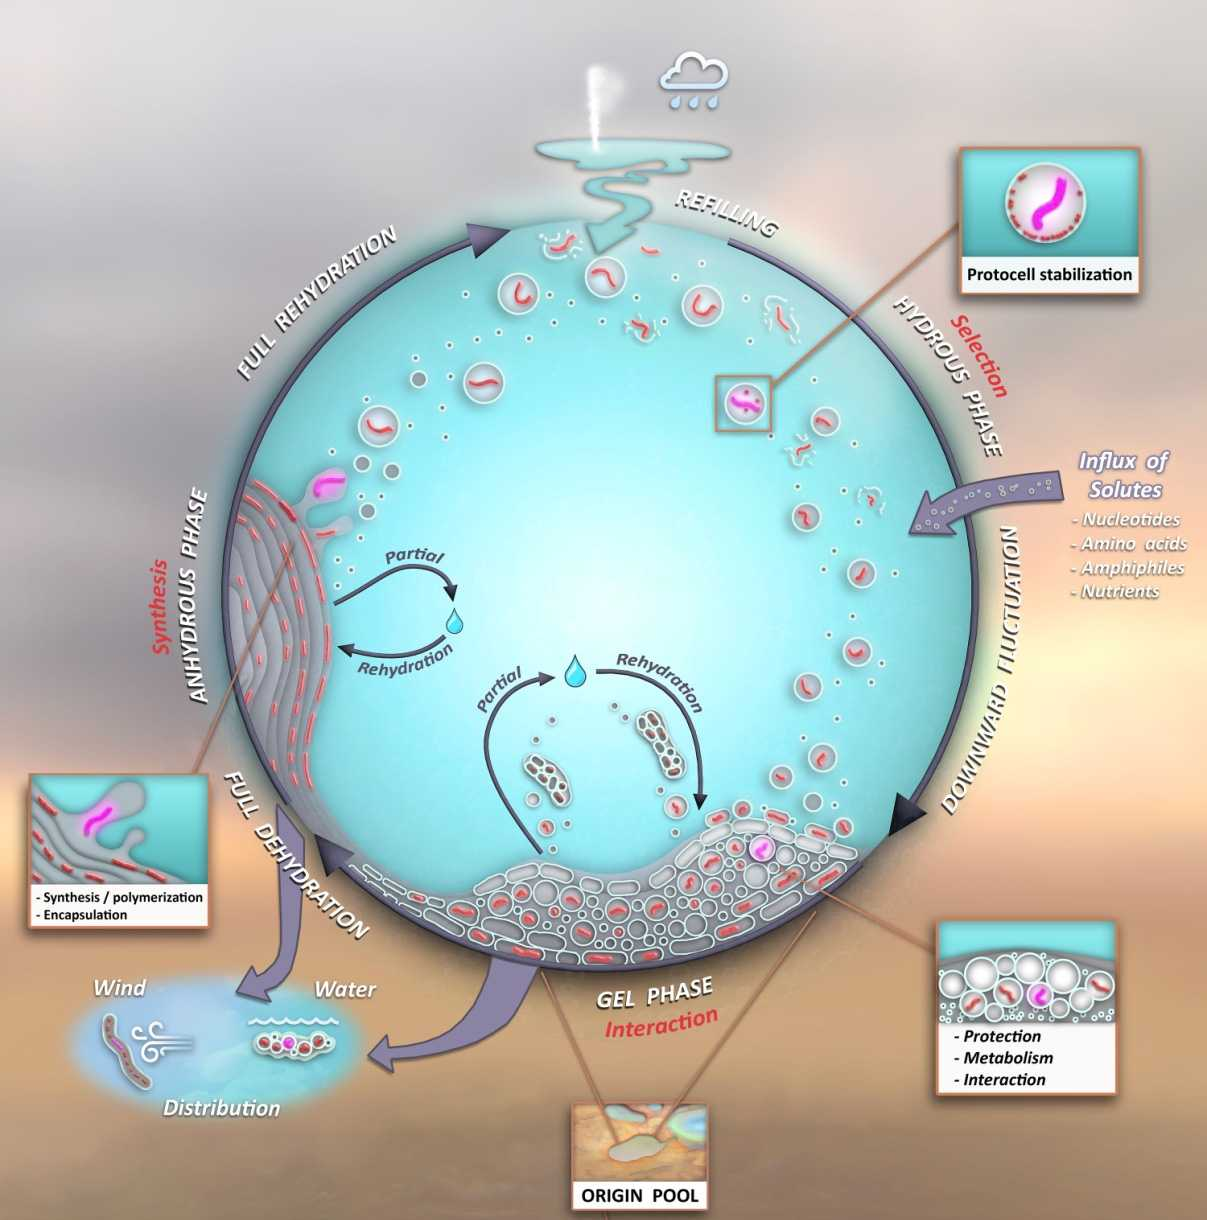
\includegraphics[width=0.8\textwidth]{WarmLittlePond}
\end{figure}
\section{Time machine}

Some physicist and engineers on a top secret project for NASA have asked you to weigh
in on their newest mission. They have a time machine, that can only be used once (and
will possibly consume an entire Universe in energy. Not ours, they assure you.). They
need to pick a time in the past to go to and look for evidence of the first biological
systems to better understand the origins of life. They will be able to bring back one
sample.
\begin{enumerate}[(a)]
	\item What time, in billions of years ago would you recommend they visit? Provide one
justification. (2 points)
	\item What type of information would you want from the early Earth conditions at that
time? Provide two types of information. (2 points)
	\item Is there a specific location/latitude you would recommend, or environment to sample
from? (1 point)
	\item What criteria would you use to tell if the sample was “alive” or once was alive? (1
point)
\end{enumerate}
\section{Phylogenic tree building}
Phylogenic tree building (instructions included in “how to generate phylogenic trees”)
\begin{enumerate}[(a)]
	\item Generate a phylogenic tree based on a single protein (or nucleotide) sequence (1
point)
	\item Generate a phylogenic tree based on the known taxonomy (1 point)
	\item Compare your protein and taxonomic trees. Do you notice any differences?
(Include at least 1 difference, or state that they are identical). (1 point)
	\item What are the challenges with building these trees? (Provide a minimum of 2
challenges) (2 points
\end{enumerate}


% glossary
\printglossaries

% bibliography go here

\bibliographystyle{unsrt}
\addcontentsline{toc}{section}{Bibliography}
\bibliography{origins,wikipedia}

\end{document}
